\documentclass[border=4pt]{standalone}
\usepackage{tikz}
\usetikzlibrary{matrix, positioning, arrows.meta}
\usepackage{xcolor}
\usepackage{amsmath, amssymb}
\definecolor{accent}{RGB}{195,30,55}
\definecolor{cool}{RGB}{31,120,180}
\newcommand{\pia}{\pi_{\alpha}}
\newcommand{\sigxi}{\sigma_{\xi}}
\newcommand{\siga}{\sigma_{\alpha}}
\newcommand{\sigr}{\sigma_{r}}
\newcommand{\sigz}{\sigma_{\zeta}}
\newcommand{\siglam}{\sigma_{\lambda}}
\newcommand{\sigs}{\sigma_{s}}
\newcommand{\kappap}{\kappa_{\text{pop}}}
\begin{document}
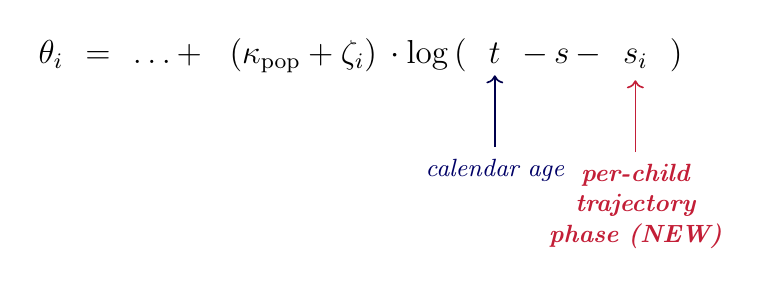
\begin{tikzpicture}[
  every node/.style={inner sep=2pt},
  ann/.style={font=\small\itshape, color=blue!40!black,
              align=center, text width=2.0cm},
  newann/.style={font=\small\itshape\bfseries, color=accent,
                 align=center, text width=2.4cm},
  arrow/.style={->, blue!30!black, semithick, shorten >=2pt, shorten <=2pt},
  newarrow/.style={->, accent, semithick, shorten >=2pt, shorten <=2pt}]
\matrix[matrix of nodes, column sep=4pt, nodes={font=\large},
        ampersand replacement=\&]{
  $\theta_i$ \&
  $=$ \&
  $\ldots +\,$ \&
  $(\kappap + \zeta_i)\,\cdot \log\,($ \&
  |[name=t]| $t$ \&
  $-\, s\, -$ \&
  |[name=si]| $s_i$ \&
  $)$ \\
};
\node[ann, below=3em of t] (at) {calendar age};
\draw[arrow] (at) -- (t);
\node[newann, below=3em of si] (asi)
  {per-child trajectory phase (NEW)};
\draw[newarrow] (asi) -- (si);
\end{tikzpicture}
\end{document}
